\section{古代东方文明}

\subsection{古代东方文明概述}
古代东方文明包括美索不达米亚,埃及,中国,印度。美索不达米亚发源于两河流域,古埃及发源于尼罗河,古代中国发源于黄河,古印度发源于印度河(相似之处:都根植于大河冲击而成的平原,以农业活动为主,称之为大河文明)。

古希腊,古罗马式西方文明的摇篮,发源于地中海东部,称之为海洋文明。

\textbf{早期文明的共同特点}
\begin{enumerate}
    \item 都是在相互孤立的状态发生的;
    \item 被西方学者称之为大河文明或灌溉文明;
    \item 城市,非农业人口;
    \item 灿烂悠久的文化:文字,神话,历法;
\end{enumerate}

\subsection{美索不达米亚文明}
美索不达米亚文明(Mesopotamia Civilization),又称两河流域文明。是指在底格里斯河和幼发拉底河两河流域之间的美索不达米亚平原(现今伊拉克境内)所发展出来的文明,是西亚最早的文明。主要由苏美尔(Sumerian)、阿卡德(Akkad)、巴比伦(Babylon)、亚述(Assyrain)等文明组成。

\begin{figure}[thbp!]
\centering
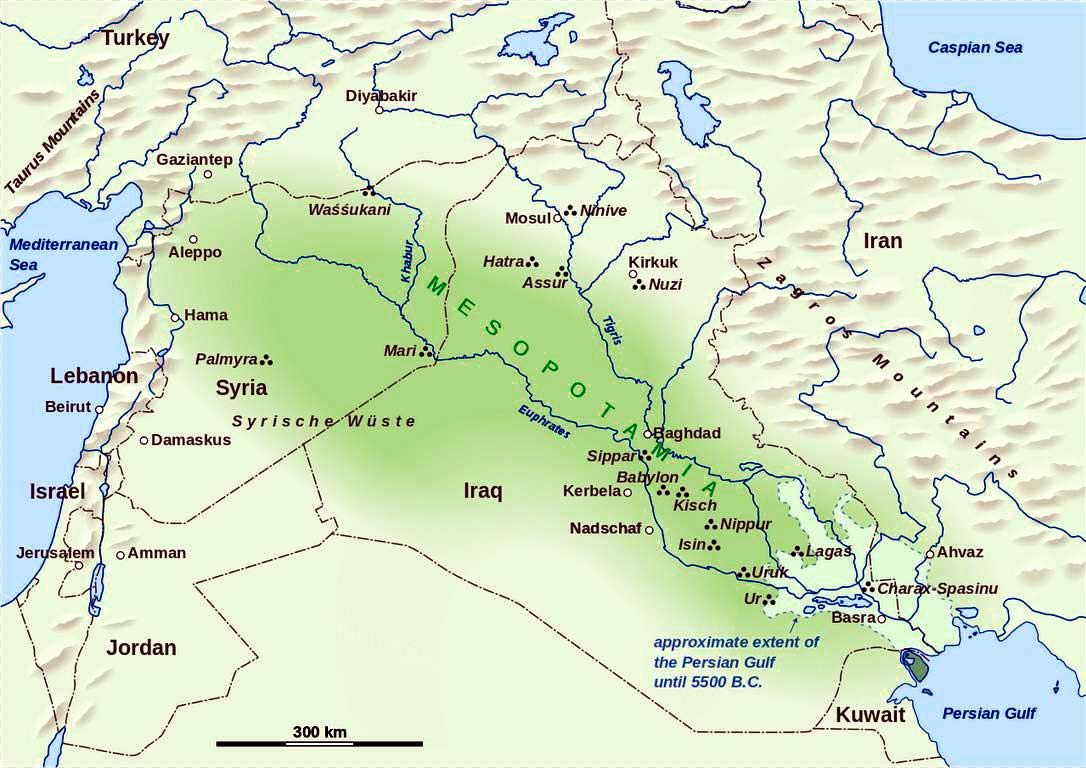
\includegraphics[width=0.8\linewidth]{figure/Map-Mesopotamian-Civilization.jpg}
\caption{Mesopotamian Civilization}
\label{fig:backphoto}
\end{figure}

\begin{figure}[thbp!]
    \centering
    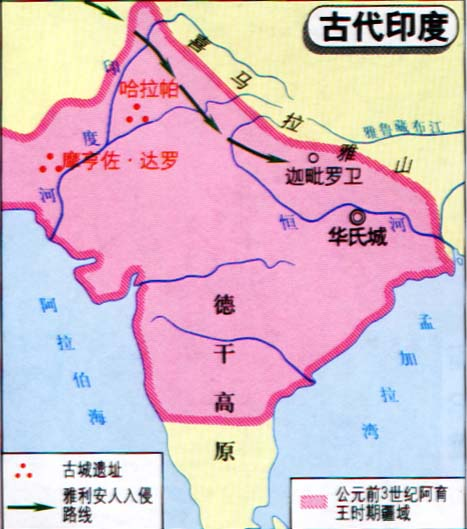
\includegraphics[width=0.8\linewidth]{figure/india.jpg}
    \caption{Mesopotamian Civilization}
    \label{fig:backphoto}
    \end{figure}

公元前3500年以后,苏美尔人在两河流域南部建立起很多奴隶制小国。公园前18世纪,古巴比伦国国王汉谟拉比统一了两河流域,建立起中央集权的奴隶制国家。

地理特点:气候干旱,底格里斯河,幼发拉底河,灌溉农业,处于“肥沃的新月地带”,两河流域不定期泛滥。

苏美尔城邦(神庙为城邦中心),信奉多神教,人与神为从属关系,建筑中最先开始使用拱劵与穹顶。对人类的贡献:发明了楔形文字,成立了培养书吏的学校;发明了车轮(由陶轮而来)。

由于两河流域地势平坦,没有天然屏障,因此常常遭到外族入侵,政权不断更迭。巴比伦时期(古巴比伦王国建立于公元前19世纪,公元前16世纪灭亡)汉谟拉比进行了专制统治(约公元前1792~公元前1750年在位),建立了强大的中央集权国家,并且编制了《汉谟拉比法典》(世界上现存的古代第一部比较完备的成文法典),以维护奴隶主阶级的利益。法典条文共282条,刻在一块巨大石柱上。法典宣扬“君权神授”。它还规定:奴隶可以买卖,还可以用来抵债。如果奴隶胆敢对主人说“你不是我的主人”,他们的耳朵就要被割掉。

国家出现后,美索不达米亚的城市社会中出现了社会等级的分化,导致了负责社会与经济结构的迅速确立,城市中生活着专业劳动者,他们生产出越来越多的高质量产品,又转而刺激了贸易的增长。不仅如此,早期的美索不达米亚还发展出独具特色的文化传统,发明了文字书写系统,组织各种宗教活动。

多产的农业经济推动了世界上最早的复杂社会的发展,大量的人群居住在城市里,在这片广大的区域里扩展他们的政治,社会,经济和文化影响。最古老的城市社会出现在公元前4千年早期的西南亚,尤其是美索不达米亚。
% 为什么出现在这,而不是其他地方
随着人口聚集在城市,需要找到解决争端的办法。争端有时存在于居住地的居民内部,有时事关整个居住地本身,这不可避免地会增加人与人或是团体之间地历史冲突。在寻找秩序地过程中,定居地农业人口承认了政治权威并在整个美索不达米亚建立了国家。国家地出现进一步促进了帝国的建立,某些国家为了扩展他们的势力,加强了自我保护能力,还将周边地区纳入自己的统治。


\subsection{腓尼基文明与希伯来文明}
腓尼基是一系列古代地中海东岸的城邦的总称,是一个海上民族。贡献:商业精神与拼音字母。腓尼基在闪米特语中为“紫色之国”,盛产紫色染料。拼音字母后被希腊学习,成为希腊字母。

希伯来文明的主要支柱是犹太教,希伯来人生活即圣经·旧约内容。

犹太教特点:
\begin{enumerate}
    \item 一神论;
    \item 反对偶像崇拜;
    \item 上帝的选民的思想;
    \item 救世主信仰“弥赛亚”;
\end{enumerate}

\subsection{古代埃及}
"Gift of the Nile" ——古希腊历史学家希罗多德

公元前15世纪,埃及国力强盛,对外征服频繁,疆土不断扩张,成为地跨亚非的大帝国。200多年以后,帝国由盛转衰。公元前6世纪,埃及被西亚的波斯灭亡。

非洲东北部,茫茫沙漠之中,尼罗河蜿蜒北流,每年定期泛滥。水退后留下肥沃的黑土,便于农业种植。约从公元前3500年开始,河流两岸陆续出现几十个奴隶制小国。约从公元前3000年,初步统一的古代埃及国家建立起来。国王自称是神的化身,他们的陵墓金字塔式权利的象征。7世纪,它成为阿拉伯帝国的一部分,古代埃及人逐渐同阿拉伯人融合。

地理特点:
\begin{enumerate}
    \item 位置相对孤立;
    \item 干旱的气候与特定的水源;
    \item 上埃及与下埃及,以孟菲斯未界;
    \item 尼罗河:水利社会;封闭,很少有外族入侵,政治格局变动不大,为大一统的中央集权国家;
    \item 贡献:象形文字,纸莎草;
\end{enumerate}

\subsection{古代印度}

约公元前2500年,印度河流域开始出现奴隶制小国,印度河流域文明兴盛于公元前2500~1700年。

古代印度是一个地理概念,指南亚次大陆,包括今天的印度,巴基斯坦,尼泊尔,孟加拉等国。

地理特点:

\begin{enumerate}
    \item 位于喜马拉雅山南侧统称为印度(为一个地区而非一个国家);
    \item 东,西,南三面环海(东面孟加拉湾,西面阿拉伯海);
\end{enumerate}

公元前14世纪雅利安人进入印度(来自中亚,自称雅利安人。白色人种,身材高大)。征服当地居民并把他们变成奴隶,先后在印度河和恒河流域建立起奴隶制国家,如图\ref{fig:india}所示。

文化特点:“种姓制度”(由雅利安人创造);种姓原意是“颜色”,因雅利安人自视高贵,与当地原住居民区分开。

特点:

\begin{enumerate}
    \item 基于“血统”的等级制度;
    \item 层次(前三等级为雅利安种姓,前二等级为统治阶级,分别对应嘴,手,腿,脚)
    \begin{enumerate}
        \item 婆罗门——祭司阶层;
        \item 刹帝利——国王,贵族武士;
        \item 吠舍——自由民;
        \item 首陀罗——被征服的土著居民
    \end{enumerate}
\end{enumerate}

因而产生规则:种族职业世袭(维护了封建社会长期的稳定性);种族内婚制;排斥外人(由不同阶层混生,不入四个等级);

积极影响:种族制度仍然存在,保证了在外邦入侵和朝代更迭时社会的稳定性。

消极影响:种族制度激化了当时的社会矛盾,并对后来的印度社会的发展带来了不良影响。


